%%
%% This is file `./samples/shortsample.tex',
%% generated with the docstrip utility.
%%
%% The original source files were:
%%
%% apa6.dtx  (with options: `shortsample')
%% ----------------------------------------------------------------------
%% 
%% apa6 - A LaTeX class for formatting documents in compliance with the
%% American Psychological Association's Publication Manual, 6th edition
%% 
%% Copyright (C) 2011-2017 by Brian D. Beitzel <brian at beitzel.com>
%% 
%% This work may be distributed and/or modified under the
%% conditions of the LaTeX Project Public License (LPPL), either
%% version 1.3c of this license or (at your option) any later
%% version.  The latest version of this license is in the file:
%% 
%% http://www.latex-project.org/lppl.txt
%% 
%% Users may freely modify these files without permission, as long as the
%% copyright line and this statement are maintained intact.
%% 
%% This work is not endorsed by, affiliated with, or probably even known
%% by, the American Psychological Association.
%% 
%% ----------------------------------------------------------------------
%% 
\documentclass[jou]{apa6}

\usepackage[american]{babel}

\usepackage{csquotes}
\usepackage[style=apa,sortcites=true,sorting=nyt,backend=biber]{biblatex}
\DeclareLanguageMapping{american}{american-apa}
\addbibresource{bibliography.bib}


%%%%%%%%%%%%%%%%%%%%%%%%%%%%%%%%%%%%%%%%
%% Discrete Structures
%% The start of RBS stuff
%%%%%%%%%%%%%%%%%%%%%%%%%%%%%%%%%%%%%%%%

% Working internal and external links in PDF
\usepackage{hyperref}
% Extra math symbols in LaTeX
\usepackage{amsmath}
\usepackage{gensymb}
\usepackage{amssymb}
% Enumerations with (a), (b), etc.
\usepackage{enumerate}

\let\OLDitemize\itemize
\renewcommand\itemize{\OLDitemize\addtolength{\itemsep}{-6pt}}

\usepackage{etoolbox}
\makeatletter
\preto{\@verbatim}{\topsep=3pt \partopsep=3pt }
\makeatother

% These sizes redefine APA for A4 paper size
\oddsidemargin 0.0in
\evensidemargin 0.0in
\textwidth 6.27in
\headheight 1.0in
\topmargin -24pt
\headheight 12pt
\headsep 12pt
\textheight 9.19in



\title{Discrete Structures (W1): Boolean Expressions}
\author{Kalvis}
\affiliation{RBS}

\leftheader{Discrete Structures (W1)}

\abstract{
You will compile a sample LaTeX document to create
math expressions easily and to satisfy the APA v6 style.
You will also manipulate Boolean expressions on paper and with the Coq.
}

\keywords{\LaTeX, APA style, Coq, Boolean expressions}

\begin{document}
\maketitle

{\em Walk-throughs} are short exercises that we do together. Their 
aim is to practice technical skills.


{\bf (W1.1)} Set up MiKTeX and Coq software.

{\bf (W1.2)} Create an APA compliant document with some math 
in LaTeX and create a PDF.

{\bf (W1.3)} Identify 6 Boolean operations. Build 
their truth tables.

{\bf (W1.4)} Translate English into propositional logic.

{\bf (W1.5)} Use precedence and associativity to draw abstract and concrete syntax trees.

{\bf (W1.6)} Run CoqIDE, check types in Coq, including atomic types, 
tuples, function types.

{\bf (W1.7)} Build truth tables for Boolean expressions.

{\bf (W1.8)} Rewrite Boolean expressions as Disjunctive Normal Form (DNF).

{\bf (W1.9)} Prove propositional tautologies with Coq.

{\bf (W1.10)} Reduce word problems to Boolean satisfiability problems.


\section{(W1.1) MiKTeX and Coq}

{\em Note.} Lab computers on the 4th floor should have these
tools installed. 
If you wish to run these tools on another Windows OS machine, 
make sure you have administrator access (for Coq) and follow 
these steps:

\begin{itemize}
\item Download MiKTeX from \url{https://miktex.org/download}
(file name {\tt basic-miktex-2.9.7269-x64.exe}). 
\item Visit \url{https://coq.inria.fr/download}. 
\item Click on "Coq 8.10.2 is out" and "8.10.2 release of Coq" links. 
Download and run {\tt coq-8.10.2-installer-windows-x86\textunderscore{}64.exe}. 
\item Create a shortcut on your desktop to run 
{\tt c:\textbackslash{}Coq\textbackslash{}bin\textbackslash{}coqide.exe}
\end{itemize}

For Linux or OS X, please ask instructor.


\section{(W1.2) Create and Compile a LaTeX Document}

\begin{itemize}
\item Get $2$ source files. 
You can visit \url{https://ctan.org/pkg/apa6} (download and
unpack ZIP, locate {\tt shortsample.tex} and 
{\tt bibliography.bib} in subdirectory "samples").
\item Also visit \url{https://bit.ly/2MX7Z09} \textendash
this directory will contain 
LaTeX files for our walk-throughs and homeworks. Then compile:
\begin{verbatim}
xelatex shortsample
biber shortsample
xelatex shortsample
\end{verbatim}
\end{itemize}

\section{(W1.3) Identify 6 Boolean operators}

Draw or review truth tables for the following Boolean operators
\parencite[see][p.4]{Rosen2019}.

\begin{itemize}
\item $A \wedge B$ (read: $A$ {\bf and} $B$).
\item $A \vee B$ (read: $A$ {\bf or} $B$). 
\item $\neg A$ (read: {\bf not} $A$).
\item $A \rightarrow B$ ({\bf if} $A$ {\bf then} $B$;
$A$ {\bf implies} $B$).
\item $A \leftrightarrow B$ ($A$ {\bf if and only if} $B$; 
$A$ {\bf equivalent to} $B$).
\item $A \oplus B$ ({\bf either} $A$ {\bf or} $B$; 
$A$ {\bf plus} $B$ {\bf modulo $2$}).
\end{itemize}



\section{(W1.4) Translate English Sentences}

Write these sentences as short Boolean expressions, 
explain the meaning of the letters used.

\begin{itemize}
\item Willy gets caught whenever he cheats.
\parencite[see][p.15, Ex24.d]{Rosen2019}.
\item My airplane flight is late iff I have to catch a connecting flight.
\parencite[see][p.16, Ex28.e]{Rosen2019}.
\item The apple trees will bloom if it stays warm for a week. 
\parencite[see][p.15, Ex25.b]{Rosen2019}.
\item The trains run late on exactly those days when I take it.
\parencite[see][p.15, Ex27.e]{Rosen2019}.
\item $x=0$ if and only if $x^2 = 0$.
\item For a quadrangle to be a parallelogram it is {\bf necessary} that
both diagonals intersect in their middle points. 
\item For a quadrangle to be a parallelogram it is {\bf sufficient} that
both diagonals intersect in their middle points. 
\item You can pay using U.S. dollars or euros.
\parencite[see][p.15, Ex27.e]{Rosen2019}.
\end{itemize}

\section{(W1.5) Use precedence and associativity}

Precedence and associativity defines how to restore omitted parentheses
in expressions with more than one operation.
Evaluate from Python command-line:

\begin{itemize}
\item $\mathtt{2+2\%3}$. Is it $\mathtt{(2+2)\%3}$ or $\mathtt{2+(2\%3)}$? 
Which is higher precedence \textendash{} addition or remainder?
\item $\mathtt{4*5**2}$. Is it $\mathtt{(4*5)**2}$ or $\mathtt{4+(5*2)}$? 
Which is higher precedence \textendash{} multiplication or raising to a power?
\item $\mathtt{31//5//2}$.  Is it $\mathtt{(31//5)//2}$ or $\mathtt{31//(5//2)}$? 
Is integer division left or right associative?
\item $\mathtt{2**3**4}$.  Is it $\mathtt{(2**3)**4}$ or $\mathtt{2**(3**4)}$? 
Is raising to a power left or right associative?
\item Is addition left or right associative?
\end{itemize}




\section{(W1.6) Run CoqIDE}

Run samples from \textcite[][p.2--8]{Bertot2010}. 


\section{(W1.7) Build Truth Tables}

Example: $(p \vee \neg(q \wedge ~r)) \rightarrow (\neg \neg r).$

{\bf (a)} Draw a truth table for the above Boolean expression. 
How many combinations can the parameters
$(p,q,r)$ have?

{\bf (b)} Enter this as a Coq proposition using logical 
connectives:
\begin{verbatim}
Variable P Q R: Prop.
Check (P \/ (Q /\ ~R)) -> (~~R).
\end{verbatim}

{\bf (c)} Define it as a function from $\mathtt{bool*bool*bool}$ 
to $\mathtt{bool}$ using prefix operations and compute 
some values:
\begin{verbatim}
Require Import Bool.
Definition myfun 
  (p:bool) (q:bool) (r:bool) : bool :=
  implb (orb p (negb (andb q (negb p)))) 
    (negb (negb r)).
Eval compute in myfun true true true.
\end{verbatim}




\section{(W1.8) Rewrite as a DNF}

For the previous Boolean expression write 
its Disjunctive Normal Form (DNF).


\section{(W1.9) Prove Tautologies with Coq}

{\em Note.} We suggest that you experiment with 
many existing proofs, try to modify them slightly. 
This will help, if you attempt proving new things.

\begin{itemize}
\item Visit \url{https://bit.ly/37EMRUq} and run 
the examples. They are identical to the CSE 191 Course Notes
\parencite[][p.12--21]{Knepley2019}.
\item Run the examples from the official Coq tutorial 
\parencite[see][]{Nahas2012}.
\item Run the examples from the {\em Software Foundations}
book, see Vol.1 Chapter ``Logic in Coq'': \url{https://bit.ly/36DtDhy}.
\end{itemize}



\section{(W1.10) Reduce to Satisfiablility}

\begin{itemize}
\item Write a Boolean expression with $4$ variables $p_1,p_2,p_3,p_4$, 
which is satisfied if and only if at least $2$ of these variables
have value {\tt true}.
\item Write a Boolean expression with $4$ variables, which is 
satisfied if and only if at least $2$ of the variables are {\tt false}.
\item How many vertices, edges and faces has the polyhedron
shown in Figure 1? Is it regular? How many Boolean variables would 
you need to write an expression that is satisfied if and only if
the polyhedron has a Hamiltonian path?
\end{itemize}

\begin{center}
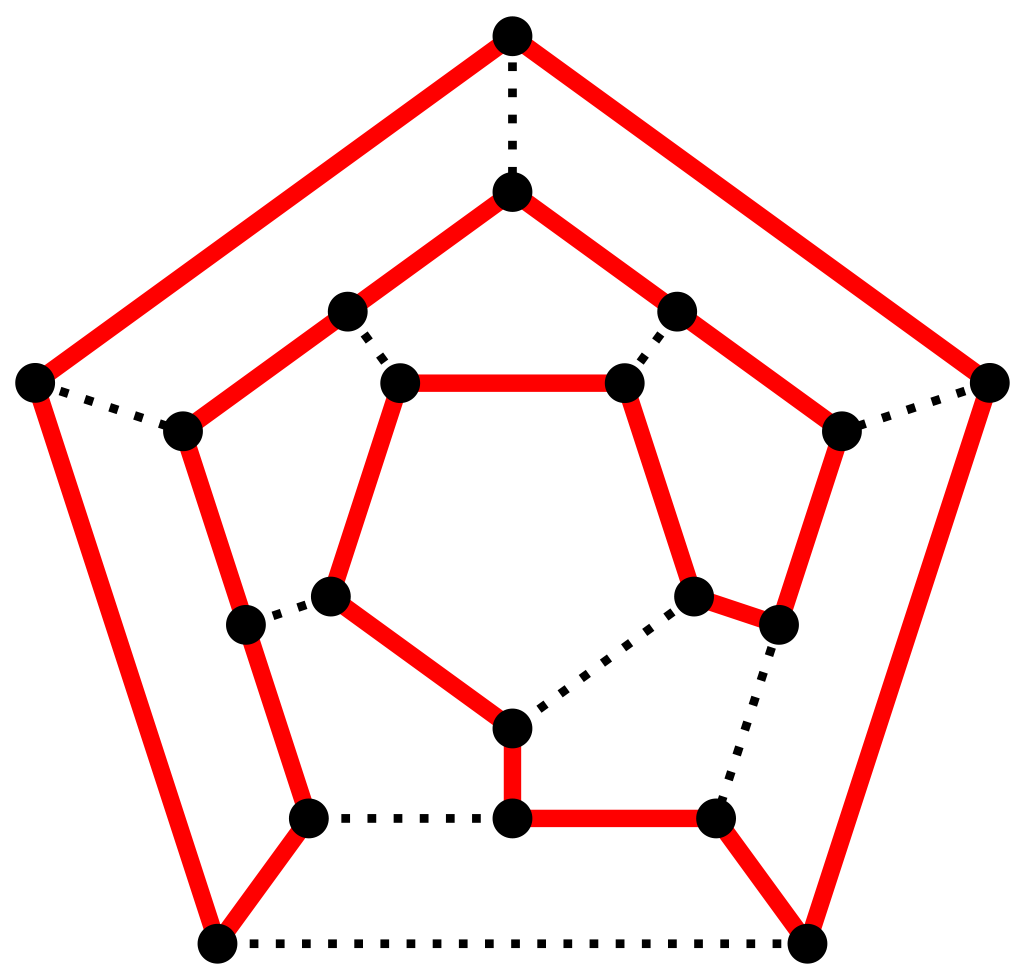
\includegraphics[width=2in]{hamiltonian-paths.png}\\
{\em Figure 1: Hamiltonian Path.}
\end{center}




\printbibliography

\end{document}



%%%%%%%%%%%%%%%%%%%%%%%%%%%%%%%%%%%%%%%%
%% End of RBS stuff
%%%%%%%%%%%%%%%%%%%%%%%%%%%%%%%%%%%%%%%%


%% 
%% Copyright (C) 2011-2017 by Brian D. Beitzel <brian at beitzel.com>
%% 
%% This work may be distributed and/or modified under the
%% conditions of the LaTeX Project Public License (LPPL), either
%% version 1.3c of this license or (at your option) any later
%% version.  The latest version of this license is in the file:
%% 
%% http://www.latex-project.org/lppl.txt
%% 
%% Users may freely modify these files without permission, as long as the
%% copyright line and this statement are maintained intact.
%% 
%% This work is not endorsed by, affiliated with, or probably even known
%% by, the American Psychological Association.
%% 
%% 
%% This work is "maintained" (as per LPPL maintenance status) by
%% Brian D. Beitzel.
%% 
%% This work consists of the file  apa6.dtx
%% and the derived files           apa6.ins,
%%                                 apa6.cls,
%%                                 apa6.pdf,
%%                                 README,
%%                                 APAamerican.txt,
%%                                 APAbritish.txt,
%%                                 APAdutch.txt,
%%                                 APAenglish.txt,
%%                                 APAgerman.txt,
%%                                 APAngerman.txt,
%%                                 APAgreek.txt,
%%                                 APAczech.txt,
%%                                 APAturkish.txt,
%%                                 APAendfloat.cfg,
%%                                 apa6.ptex,
%%                                 TeX2WordForapa6.bas,
%%                                 Figure1.pdf,
%%                                 shortsample.tex,
%%                                 longsample.tex, and
%%                                 bibliography.bib.
%% 
%%
%% End of file `./samples/shortsample.tex'.
